\section{Hardware-támogatás}

A MATLAB 2013b verziójától elérhető direkt hardware-támogatás az STM32F4 Discovery fejlesztőkártyához, melyet a MATLAB Hardware Support oldaláról tölthetünk le. A támogatás segítségével villámgyorsan tesztelhetjük az elkészített szoftvert, soros kábel segítségével pedig akár Processor-in-the-Loop tesztet is végrehajthatunk.

\subsection{Gyors Prototípustervezés}

A RobonAUT elsősorban gyors prototípustervezési munkát igényel. Rövid idő alatt, minél hatékonyabb párhuzamosítással és a lehető legkevesebb teszteléssel kell sok funkcióval rendelkező, többé-kevésbé megbízható rendszert építeni. A magas és az alacsony szintű irányítás fejlesztése teljesen párhuzamosan zajlik, ha megfelelően kiaknázzuk a lehetőségeket.

\paragraph{Példa} Készítsünk Simulinkben egy LED-villogtató programot 5 perc alatt!

Miután feltelepítettük a support package-et\footnote{Ekkor indul a stopper}, hozzunk létre egy új Simulink modellt, majd húzzuk be az \textbf{Embedded Coder Support Package for STMF4-Discovery Board} library-ből a szükséges blokkokat. Az ábrán látható módon állítuk össze a kapcsolást, majd konfiguráljuk a modellt az 1. részben leírtakhoz hasonlóan, de most a \textbf{Code Generation} menüben \textbf{Target Hardware}-nek válasszuk az \verb!STM32F4-Discovery!-t, valamint ne csak kódot generáljunk (Pipa ki a \textbf{Generate code only} checkbox-ból).\footnote{Cheat sheet újoncoknak: A \texttt{Constant} blokk signal type-ját  \texttt{boolean}-re, a  \texttt{Pulse Generator} Pulse type-ját pedig  \texttt{Sample based}-re kell állítani. A blokkokról pedig senki sem tudja, hogy melyik almenüben vannak, érdemes használni a keresőt. Ne felejtsük el a GPIO blokkok konfigurálását sem! Ha semmiképpen sem akar működni, akkor a kész modell letölthető \href{http://www.mathworks.com/matlabcentral/fileexchange/45953-stm32f4-discovery-led-blinker}{\texttt{innen}}.}

\begin{figure}[!ht]
    \centering
    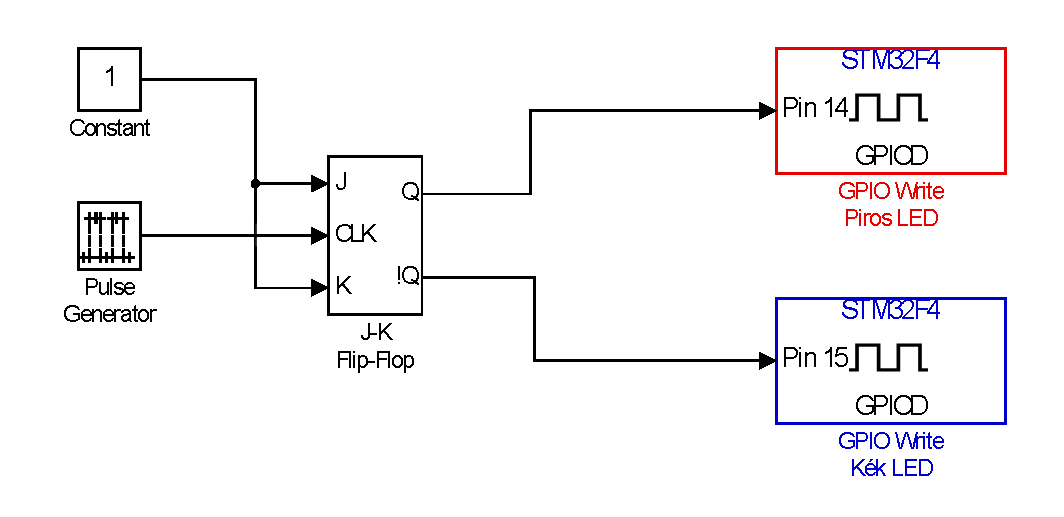
\includegraphics[width=0.9\linewidth]{img/stmblink}
    \caption{LED villogtató Simulink-modell}
    \label{fig:stmblink}
\end{figure}

A teljes rendszert a \textbf{Code} menü \textbf{C/C++ Code} menüpontjából tudjuk buildelni. Ha mindent jól csináltunk, a jutalmunk a végén egy \verb!.hex!, egy \verb!.elf! és egy \verb!.bin! file lesz a Working Directory-ben. Ezután az \texttt{STM ST-LINK Utility} segítségével felprogramozhatjuk a kártyát a generált fileok segítségével. Természetesen nem csak a ledeket tudjuk villogtatni, hanem az összes GPIO-t, gombot és analóg I/O-t kezelni tudjuk tetszőlegesen bonyolult modell köré építve. A GPIO Read és Write blokkok beállításához az \texttt{ST-Microelectronics} megfelelő segédletet nyújt\cite{usermanual}.

Hasonló elv alapján épült fel egy standard servo jeleket feldolgozó projekt is, melyet egy távirányítós autó végfokozatának PWM-es vezérlésére használtam.A Simulink modell szintén letölthető \href{http://www.mathworks.com/matlabcentral/fileexchange/46221-rc-car-control-with-stm32f4-discovery-programmed-by-matlab}{\texttt{innen}}, és mélyebb betekintést ad a modell alapú tervezés nyújtotta lehetőségekbe. Egy ilyen feladat elkészítése is inkább munkapercekben, mint -órákban mérhető.
Korábban említettük, hogy akár PIL tesztelésre is lehetőség van. Ebben a dokumentumban erre az alkalmazási területre nem térünk ki, de egy későbbi bővített kiadásban előfordulhat, ha igény mutatkozik a témára.